% Draft manuscript. For IEEE submission replace the next line with
%   \documentclass[conference]{IEEEtran}
% (IEEEtran.cls was not available in the build environment; only standard commands are used.)
\documentclass[10pt,twocolumn]{article}
\usepackage[margin=1.8cm]{geometry}
\usepackage{booktabs,graphicx,amsmath,amssymb,cite,hyperref}
\graphicspath{{figures/}}
\title{Adaptive Quantum-Safe Security and Privacy for Healthcare Data}
\author{Jose Rohit M and Karthikeyan Jayaraman\\ SCORE, Vellore Institute of Technology, Vellore, India}
\date{Draft, October 2026}
\begin{document}
\maketitle

\begin{abstract}
Hospitals must protect patient data against future quantum attacks and also de-identify it for secondary use, yet stronger protection costs time: NIST-standardised post-quantum objects (ML-KEM, ML-DSA) are one to two orders of magnitude larger than classical ones, which threatens the roughly 200\,ms delivery SLA of streaming IoMT telemetry on congested links. Existing work treats these concerns separately: PQC migration and crypto-agility studies address algorithms and processes, runtime-adaptive IoMT security does not adapt data privacy, and adaptive differential-privacy controllers have no cryptographic dimension. We present Agile-HQ-PQC, a gateway whose controller, CADA-AASM, selects the strongest protection the network can currently afford---transport cryptography \emph{and} privacy parameters together---from a live latency budget $L=200-\mathrm{RTT}-0.5\,\mathrm{CPU}$, with a persistence filter against cipher flapping and a hard floor (NIST Category~3) for raw clinical telemetry. In a 30-trial paired evaluation under an \emph{emulated} congestion model, steering reduced SLA violations during stress relative to static Tier~5 (clinical $7.4\%\to4.1\%$, research $6.9\%\to2.9\%$, both $p<10^{-4}$), was statistically indistinguishable from static Tier~3 while running the strongest suite in calm periods, and cut tier changes by $65\%$. The benefit is concentrated on constrained links ($-45$\,pp at 1\,Mbps) and vanishes at $\ge5$\,Mbps; batch ML-DSA signing alone removes most of the latency problem. A real-link validation (network namespaces, kernel bandwidth shaping, real TCP) does \emph{not} reproduce the emulated gain at $\ge2$\,Mbit/s: adaptation matters only on very thin links, where static Tier~5 fails outright but a well-chosen static Tier~3 does as well. We report these negative results alongside the positive ones.
\end{abstract}

\section{Introduction}
Adversaries can record encrypted hospital traffic today and decrypt it once a cryptanalytically relevant quantum computer exists (``harvest now, decrypt later''); clinical data such as genomics has a confidentiality horizon of decades, so migration to PQC cannot wait~\cite{fips203,fips204}. PQC has an operational cost, however. An ML-DSA-87 signature is 4\,627\,bytes (Ed25519: 64) and an ML-KEM-1024 ciphertext is 1\,568\,bytes (X25519: 32), so a signed telemetry packet spans several Ethernet frames, increasing serialisation time and exposure to loss exactly when a hospital network is congested. Streaming ICU telemetry tolerates about 200\,ms end to end.

Separately, data leaving the clinical system for secondary use must be de-identified: differential privacy~\cite{dwork} for numeric streams and $(K,L)$-anonymity~\cite{sweeney,ldiv} for tabular records. Section~\ref{sec:related} shows that, in the literature we reviewed, no work adapts transport cryptography and data-privacy strength together under a latency constraint with a compliance floor.

\textbf{Research question.} Can transport security and data privacy be treated as one trade-off, steered by the network's remaining latency budget, without ever dropping raw patient data below a safe minimum?

\textbf{Contributions.} (i) \emph{A joint model}: three protection levels (High/Medium/Low; Tier~5/3/1) that bind KEM, signature, AEAD, $\varepsilon$, $K$ and $L$ together and are chosen by a single latency-budget controller (CADA-AASM). (ii) \emph{A safe adaptive policy}: persistence filtering against flapping and a Category-3 floor for raw PHI; researcher exports additionally enforce $K\ge5$, $L\ge3$. (iii) \emph{An honest evaluation}: 30 paired trials, ablations and a bandwidth$\times$loss sweep showing where adaptation helps (constrained links) and where it does not ($\ge5$\,Mbps, or with batch signing). The open implementation, operator console, tamper lab and tamper-evident audit log support these contributions but are not claimed as research novelty.

\section{Related Work}\label{sec:related}
We read in full 18 papers from IEEE Xplore published from 2023 to 2026~\cite{ieee04_elhadedy2024,ieee05_yadav2023,ieee06_sinaga2025,ieee07_santos2026,ieee08_karthikeyan2023,ieee09_zhukabayeva2024,ieee10_aydeger2026,ieee11_ojetunde2025,ieee12_lokesh2025,ieee13_rubiogarcia2023,ieee14_catoni2025,ieee15_rigon2025,ieee16_reazaei2026,ieee17_he2024,ieee18_yu2024,ieee19_zhang2023,ieee20_lyu2025,ieee21_birajdar2025}, together with the NIST guidance~\cite{cswp39}, and checked novelty against seven non-IEEE works~\cite{alif,kampanakis,qpradax,adaptiveqke,caap,alpine,zaman}. The search was a single reviewer working on IEEE Xplore only, so it is not a systematic review, and the gap below holds for these works, not for all published work.

\textbf{PQC for healthcare.} El-Hadedy et al.~\cite{ieee04_elhadedy2024} run Kyber and ASCON on a K3S cluster of small ARM boards for IoMT; Kyber512 encapsulation took 3\,464\,$\mu$s and the algorithm is chosen once per deployment. Yadav et al.~\cite{ieee05_yadav2023} give a Ring-LWE and PUF authenticated key exchange with security and cost analysis only. Karthikeyan~\cite{ieee08_karthikeyan2023} combines RSA, Twofish and NTRUEncrypt (not a NIST-standardised scheme) for medical images, and Zhukabayeva et al.~\cite{ieee09_zhukabayeva2024} evaluate hash-based PQC on Hyperledger Fabric by discrete-event simulation. All four protect transport or storage with fixed settings and do no network adaptation.

\textbf{PQC cost on networks.} Santos et al.~\cite{ieee07_santos2026} measured ML-KEM-768 and ML-DSA-65 hybrid TLS for MQTT at 212\,ms connection setup against 44\,ms classical (4.7 times) and found the cost was computation, not bandwidth. Ojetunde et al.~\cite{ieee11_ojetunde2025}, Lokesh~\cite{ieee12_lokesh2025} (14.1\,ms handshake on Raspberry Pi~3), Rubio Garcia et al.~\cite{ieee13_rubiogarcia2023} (about 68\% more handshake time for a triple hybrid) and Rigon et al.~\cite{ieee15_rigon2025} (ML-KEM most efficient in QUIC) each measure one fixed configuration at a time; Reazaei et al.~\cite{ieee16_reazaei2026} review ML-KEM, BIKE and HQC without a network test. Catoni et al.~\cite{ieee14_catoni2025} show TLS~1.3 resumption cuts connection cost by up to 73\%. Together with~\cite{ieee07_santos2026} this points to long-lived sessions, which fits our make-before-break re-keying, and exposes a limit of our real-link test: it does not charge post-quantum computation to latency.

\textbf{Adaptive PQC.} Only two of the 18 papers adapt post-quantum settings at run time. Sinaga et al.~\cite{ieee06_sinaga2025} tune Kyber and Saber parameters by rules from CPU and RAM load on one device, with no network and no privacy. Aydeger and Carvalho~\cite{ieee10_aydeger2026} add cryptographic agility to simulated UAV swarms; at 50 UAVs static high security met 7.5\% of deadlines while agile and static low met 90\%, but their security floors are soft and may be dropped under load. Neither is for healthcare, neither adapts privacy, and neither is tested on a shaped link. Run-time PQC selection also appears outside IEEE Xplore~\cite{qpradax,adaptiveqke,caap}, so we do not claim it.

\textbf{Privacy for medical data.} Zhang et al.~\cite{ieee19_zhang2023} combine lightweight attribute-based encryption with differential privacy for medical IoT under a static policy. Lyu et al.~\cite{ieee20_lyu2025} generate synthetic medical data with budgets set by Shapley value and entropy, once per dataset.

\textbf{Adaptive privacy.} He et al.~\cite{ieee17_he2024} adapt local-DP clipping per layer inside clustered federated learning on image data; Yu et al.~\cite{ieee18_yu2024} set noise and budget from gradient components in medical federated learning; Birajdar et al.~\cite{ieee21_birajdar2025} propose a dynamic budget framework with R\'enyi accounting but no experiments. These react to training, not to network latency, and \cite{ieee21_birajdar2025} is theory only; Lyu et al.~\cite{ieee20_lyu2025} set their budgets once per dataset, so they do not adapt at run time. None touches the transport cipher. Adaptive or data-driven privacy budgets also exist~\cite{ieee18_yu2024,ieee20_lyu2025,ieee21_birajdar2025,alpine}, so we do not claim them either.

\textbf{Research gap.} Of the 18 papers, none sets a differential-privacy or anonymity parameter together with a post-quantum suite. Our claimed gap is joint control of transport cryptography and privacy through one latency budget, with a hard floor for raw clinical data, evaluated on emulated and real shaped links; a 2026 survey lists this direction as open~\cite{zaman}. Table~\ref{tab:gap} summarises the comparison.

\begin{table*}[t]\centering\small
\caption{Positioning of the 18 surveyed IEEE Xplore papers against this work.}\label{tab:gap}
\begin{tabular}{llllll}\toprule
Work & Healthcare & Post-quantum & Privacy (DP or anonymity) & Adapts at run time & Tested on a network\\\midrule
\cite{ieee04_elhadedy2024} & yes & yes & no & no & cluster, compute only\\
\cite{ieee05_yadav2023} & yes & yes & authentication privacy & no & analysis\\
\cite{ieee06_sinaga2025} & no & yes & no & yes, CPU and RAM rules & no\\
\cite{ieee07_santos2026} & no & yes & no & no & emulated\\
\cite{ieee08_karthikeyan2023} & yes & yes (NTRU) & no & no & no\\
\cite{ieee09_zhukabayeva2024} & yes & yes & no & no & simulated\\
\cite{ieee10_aydeger2026} & no & yes & no & yes, soft floors & simulated\\
\cite{ieee11_ojetunde2025} & no & yes & no & no & wireless test\\
\cite{ieee12_lokesh2025} & no & yes & no & no & hardware, loss tested\\
\cite{ieee13_rubiogarcia2023} & no & yes & no & no & experimental network\\
\cite{ieee14_catoni2025} & no & yes & no & no & several conditions\\
\cite{ieee15_rigon2025} & no & yes & no & no & controlled\\
\cite{ieee16_reazaei2026} & no & yes & no & no & review\\
\cite{ieee17_he2024} & no & no & yes & yes, in training & no\\
\cite{ieee18_yu2024} & yes & no & yes & yes, in training & no\\
\cite{ieee19_zhang2023} & yes & no & yes & no & simulated\\
\cite{ieee20_lyu2025} & yes & no & yes & no (budgets set once per dataset) & no\\
\cite{ieee21_birajdar2025} & yes & no & yes & yes, theory only & no\\
\midrule
\textbf{This work} & \textbf{yes} & \textbf{yes} & \textbf{yes} & \textbf{yes, from latency budget} & \textbf{emulated and real shaped link}\\\bottomrule
\end{tabular}\end{table*}

\section{Design}
\textbf{Budget and steering.} Each cycle the gateway measures RTT $R$ and CPU utilisation $C$ (\%) and computes $L=200-R-0.5C$. $L>80$\,ms selects Tier~5 (ML-KEM-1024, ML-DSA-87, AES-256-GCM, $\varepsilon=0.1$, $K=5$, $L_{div}=3$); $40<L\le80$ Tier~3 (ML-KEM-768, ML-DSA-65, AES-256-GCM, $0.5$, 3, 2); $L\le40$ Tier~1 (ML-KEM-512, ML-DSA-44, ChaCha20-Poly1305, $1.0$, 2, 2). A transition is committed only after the same different target appears on three consecutive cycles.

\textbf{Dual-domain policy.} The agile tier governs the de-identified research stream: Laplace noise scale $\Delta/\varepsilon$ on physiological samples and Mondrian~\cite{mondrian} $(K,L)$-partitioning on EHR records. The raw clinical stream uses $\max(\text{agile},3)$, so PHI is never protected below NIST Category~3 irrespective of congestion. Researcher exports additionally enforce $K\ge5$, $L\ge3$ and are re-verified independently before release.

\textbf{Hybrid channel.} Key establishment combines X25519 and ML-KEM by HKDF over the concatenated secrets salted with the transcript hash; the server signs the transcript with Ed25519 \emph{and} ML-DSA and both must verify. Packets are AEAD-protected with tier, session and sequence number as associated data and carry an Ed25519 signature; an ML-DSA signature over a hash chain of the epoch is attached every $E$ packets ($E=1$: per-packet PQ signature; $E=8$: batch signing). Re-keying on a tier change is make-before-break.

\section{Implementation}
Python; \texttt{kyber-py}/\texttt{dilithium-py} (FIPS 203/204 reference code, not constant-time) and \texttt{cryptography}; Flask/Socket.IO console with role-based JWT access (admin, auditor, researcher, operator); hash-chained, HMAC-protected audit log; 59 automated tests covering controller invariants, crypto rejection of every tampered field, $(K,L)$ verification and RBAC.

\section{Evaluation}
\textbf{What is modelled.} Cryptography, packet sizes, anonymisation and control logic are executed for real. Congestion is \emph{emulated}: injected RTT, CPU load, loss and bandwidth, and a delivery model $\text{latency}=R+\text{serialisation}+\text{queueing}\,(\text{fragments}-1)+\text{one RTO on loss}$. PQ compute is not charged to per-packet latency (pure-Python code would measure the interpreter); only wire bytes are. Results therefore characterise the mechanism, not a hospital network.

\textbf{Protocol.} 30 paired seeds; each trial has 60 cycles: calm(12), moderate(10), heavy(10), severe(12), calm(16). Baselines: static T5, static T3, CADA without hysteresis, each with per-packet PQ signatures; plus batch-signing variants. Paired Wilcoxon signed-rank tests.

\begin{table*}[t]\centering\caption{Staged-stress evaluation, 30 paired trials, mean $\pm$ 95\% CI.}\label{tab:main}\small
\begin{tabular}{lrrrrrr}\toprule
Metric & Static T5 & Static T3 & CADA, no hyst. & CADA-AASM & T5 + batch & CADA + batch \\\midrule
Clinical viol.\ (stress) & 7.4\% $\pm$ 1.5 & 3.9\% $\pm$ 1.0 & 3.9\% $\pm$ 1.0 & 4.1\% $\pm$ 1.1 & 1.1\% $\pm$ 0.5 & 1.1\% $\pm$ 0.5 \\
Research viol.\ (stress) & 6.9\% $\pm$ 1.6 & 3.5\% $\pm$ 1.3 & 2.8\% $\pm$ 1.2 & 2.9\% $\pm$ 1.1 & 0.8\% $\pm$ 0.6 & 0.7\% $\pm$ 0.5 \\
Clinical p95 (ms) & 195.7 $\pm$ 2.5 & 187.3 $\pm$ 1.9 & 187.4 $\pm$ 1.9 & 187.7 $\pm$ 2.1 & 172.6 $\pm$ 1.6 & 173.7 $\pm$ 1.7 \\
Research p95 (ms) & 197.8 $\pm$ 7.8 & 187.1 $\pm$ 2.7 & 185.1 $\pm$ 3.5 & 184.2 $\pm$ 2.8 & 172.2 $\pm$ 1.7 & 173.0 $\pm$ 1.9 \\
Mean wire bytes & 5030.2 $\pm$ 0.1 & 3712.2 $\pm$ 0.1 & 4546.9 $\pm$ 0.1 & 4609.9 $\pm$ 21.3 & 943.0 $\pm$ 0.1 & 821.6 $\pm$ 4.2 \\
Handshakes/trial & 2.0 $\pm$ 0.0 & 2.0 $\pm$ 0.0 & 10.9 $\pm$ 0.6 & 6.4 $\pm$ 0.2 & 2.0 $\pm$ 0.0 & 6.4 $\pm$ 0.2 \\
Tier changes/trial & 0.0 $\pm$ 0.0 & 0.0 $\pm$ 0.0 & 6.9 $\pm$ 0.6 & 2.4 $\pm$ 0.2 & 0.0 $\pm$ 0.0 & 2.4 $\pm$ 0.2 \\
\bottomrule\end{tabular}\end{table*}

\begin{table}[t]\centering\caption{Paired Wilcoxon tests, CADA-AASM minus baseline (per-packet PQ signatures).}\label{tab:tests}\small
\begin{tabular}{llrr}\toprule
Baseline & Metric & mean diff & Wilcoxon $p$ \\\midrule
T5 & clin.\ viol.\ (pp) & -3.33 & 6.0e-05 \\
T5 & res.\ viol.\ (pp) & -3.96 & 2.9e-05 \\
T5 & res.\ p95 (ms) & -13.54 & 1.9e-09 \\
T5 & tier changes & +2.40 & 5.9e-07 \\
T3 & clin.\ viol.\ (pp) & +0.21 & 1.6e-01 \\
T3 & res.\ viol.\ (pp) & -0.62 & 5.8e-02 \\
T3 & res.\ p95 (ms) & -2.84 & 2.0e-07 \\
T3 & tier changes & +2.40 & 5.9e-07 \\
no hyst. & clin.\ viol.\ (pp) & +0.21 & 1.6e-01 \\
no hyst. & res.\ viol.\ (pp) & +0.10 & 7.1e-01 \\
no hyst. & res.\ p95 (ms) & -0.84 & 7.2e-01 \\
no hyst. & tier changes & -4.47 & 2.3e-06 \\
\bottomrule\end{tabular}\end{table}

\begin{table}[t]\centering\caption{Sweep: CADA minus static-T5 SLA-violation rate (percentage points), constant severe RTT/CPU stress.}\label{tab:sweep}\small
\begin{tabular}{lrrrr}\toprule
loss $\backslash$ bw & 20 Mbps & 5 Mbps & 2 Mbps & 1 Mbps \\\midrule
0\% & +0.0 & +0.0 & -2.1 & -44.8 \\
0.5\% & +0.0 & +0.0 & -4.2 & -45.8 \\
1\% & -1.0 & -1.0 & -4.7 & -44.3 \\
2\% & -1.0 & -1.0 & -4.7 & -43.2 \\
\bottomrule\end{tabular}\end{table}


\begin{figure}[t]\centering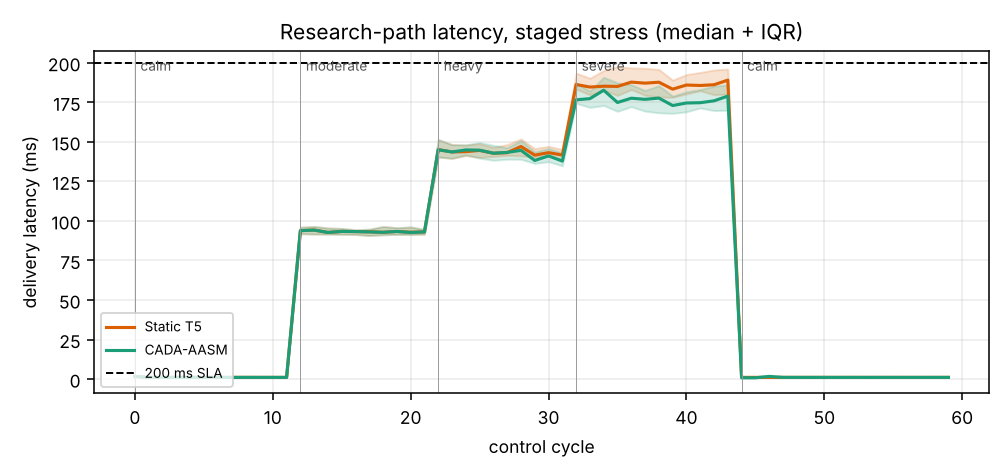
\includegraphics[width=\columnwidth]{fig1.png}\caption{Research-path latency under staged stress (median, IQR over 30 trials).}\label{fig:lat}\end{figure}
\begin{figure}[t]\centering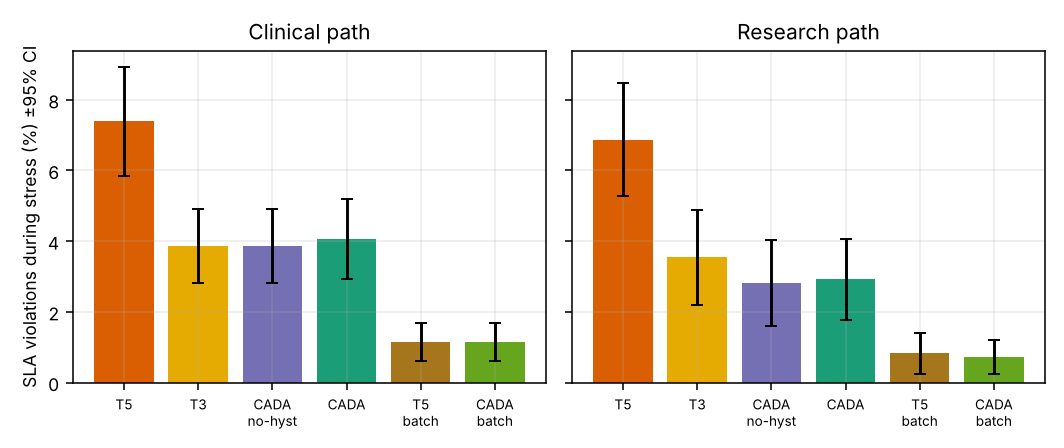
\includegraphics[width=\columnwidth]{fig2.png}\caption{SLA violations during stress with 95\% CI.}\label{fig:viol}\end{figure}
\begin{figure}[t]\centering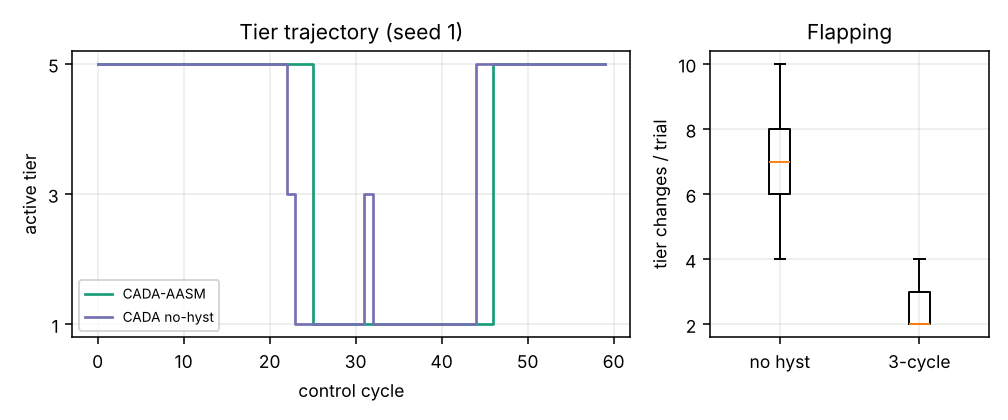
\includegraphics[width=\columnwidth]{fig3.png}\caption{Tier trajectory and flapping with and without the persistence filter.}\label{fig:flap}\end{figure}
\begin{figure}[t]\centering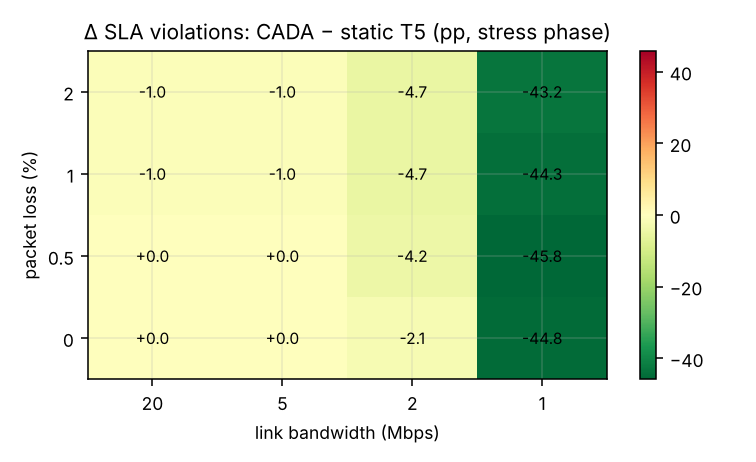
\includegraphics[width=0.9\columnwidth]{fig5.png}\caption{Where steering helps: bandwidth$\times$loss sweep.}\label{fig:sweep}\end{figure}

\section{Results and Discussion}
\textbf{Against static Tier~5} (per-packet PQ signatures), steering lowered SLA violations during stress from 7.4\% to 4.1\% (clinical) and 6.9\% to 2.9\% (research) and p95 latency by 8--14\,ms (Table~\ref{tab:main},\ref{tab:tests}, Figs.~\ref{fig:lat},\ref{fig:viol}), at the cost of about 4.4 extra handshakes per trial.

\textbf{Against static Tier~3} the violation rates were not significantly different (clinical $p=0.16$, research $p=0.058$). The value of steering here is not lower latency than a permanently weaker suite but obtaining the strongest suite and the strongest privacy parameters (mean $\varepsilon=0.37$, $K=4.1$ over the trial) whenever the budget allows, instead of a fixed compromise.

\textbf{Hysteresis} cut tier changes from 6.9 to 2.4 per trial and handshakes from 10.9 to 6.4 with no significant change in violations. We did not observe a latency benefit from hysteresis; its benefit is stability and re-key cost.

\textbf{The clinical floor} held in all trials (minimum clinical tier 3). Because the floor prevents the clinical path from reaching Tier~1, clinical violations under steering equal those of static Tier~3 ($4.1\%$ vs $3.9\%$); this is the price of the compliance invariant.

\textbf{Negative result: batch signing.} Amortising the ML-DSA signature over eight packets reduced mean wire size from about 5.0\,kB to 0.9\,kB and violations to 1.1\% with or without steering (Table~\ref{tab:main}); with batch signing, steering showed no significant latency benefit (Table~\ref{tab:tests}) and slightly worse clinical p95 ($+1.1$\,ms, $p=0.0497$). Thus the latency argument for steering depends on the signature strategy; the privacy-adaptation argument is independent of it.

\textbf{Sensitivity.} Steering helped little or not at all at $\ge5$\,Mbps, modestly at 2\,Mbps ($-2$ to $-5$\,pp) and strongly at 1\,Mbps ($\approx-45$\,pp, Table~\ref{tab:sweep}), where a 5\,kB packet cannot be serialised inside the budget. The mechanism is therefore most relevant to bandwidth-constrained IoMT links (cellular, low-power radio, congested Wi-Fi).

\textbf{Real-link validation.} To test the emulated model we ran the same staged schedule over two Linux network namespaces joined by a veth pair with kernel token-bucket shaping, real TCP, the project's actual packet bytes, an echo-probe RTT over the shaped link and real CPU load (4 repetitions per cell; propagation delay is a stated receiver hold and loss is not modelled because kernel netem was unavailable). Results are in Fig.~\ref{fig:real}. With staged stress no configuration violated the SLA and static Tier~5 had only $\approx5.6$\,ms higher p95 latency than CADA or Tier~3 (equal with batch signing): \emph{the emulated gain over static Tier~5 is not reproduced on a real link at $\ge2$\,Mbit/s}, so it was driven by the emulator's fragment-queueing and loss terms rather than wire bytes alone. Under constant severe stress, size matters only at the lowest rates: at 0.5\,Mbit/s static Tier~5 violated the SLA on every cycle, CADA on 13\% (it starts at Tier~5 and needs three cycles and a re-key to step down) and static Tier~3 on none; at 1\,Mbit/s CADA (3.3\%) was slightly worse than both statics. Native liboqs timings (ML-DSA-65 sign $\approx0.09$\,ms versus $\approx94$\,ms for the pure-Python code) confirm that wire size, not compute, is the cost that matters. With four pairs the smallest attainable Wilcoxon $p$ is 0.125, so these are descriptive results.

\begin{figure}[t]\centering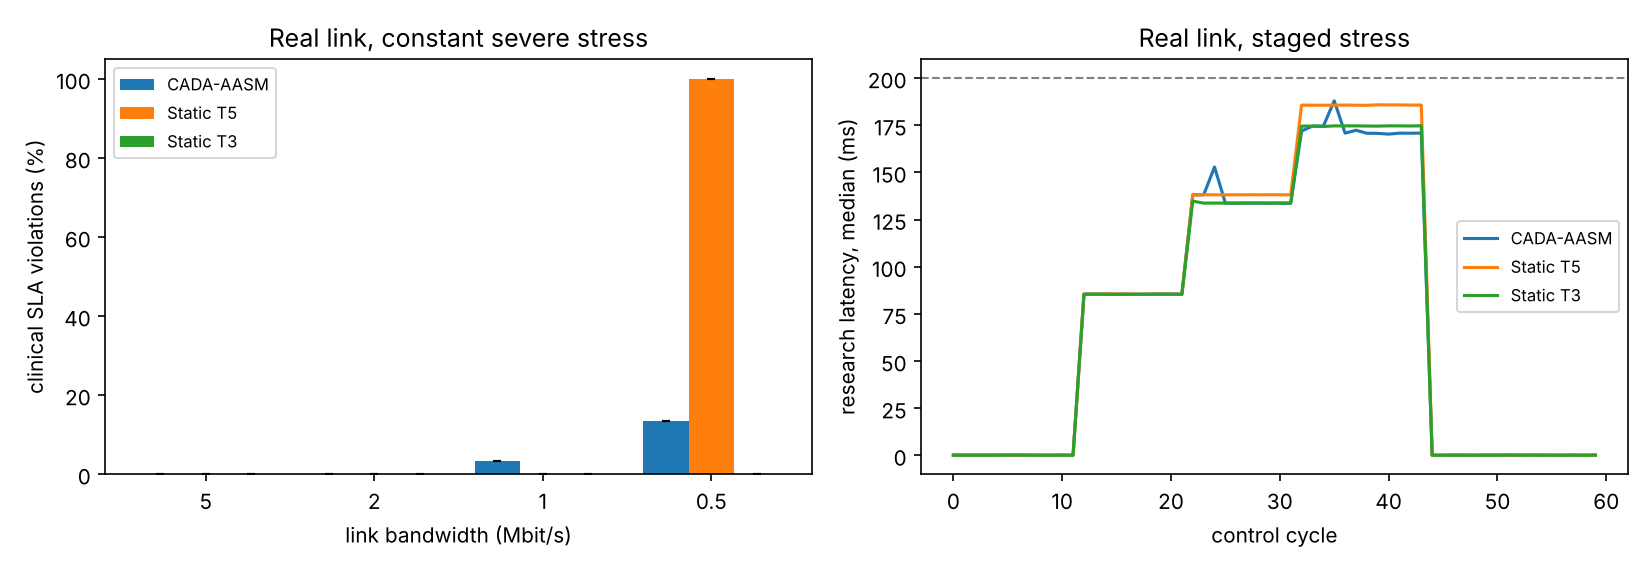
\includegraphics[width=\columnwidth]{fig6.png}\caption{Real-link validation (namespaces + kernel tbf). Left: clinical SLA violations under constant severe stress vs bandwidth. Right: median research latency under staged stress.}\label{fig:real}\end{figure}

\section{Limitations}
In the main evaluation congestion and the latency model are assumptions (the real-link validation covers bandwidth shaping and real RTT/CPU only); PQ code is a non-constant-time reference implementation; stress presets are author-chosen; Laplace sensitivity $\Delta$ is a modelling choice; Mondrian gives only $k$-anonymity and distinct $\ell$-diversity; variable privacy parameters tied to network state require data-governance review; the related-work comparison is from abstracts and available text, not a systematic review or prior-art search. Kernel \texttt{netem} packet loss and delay, a multi-host virtual-machine testbed with a native liboqs TLS stack, and a user study with clinicians are future work.

\section{Conclusion}
Treating transport strength and privacy strength as one latency-budget-driven control problem is implementable, keeps a compliance floor for raw PHI, and measurably reduces SLA violations relative to static maximum security on constrained links, but under our model it does not beat a well-chosen static Tier~3 on latency and becomes latency-neutral once PQ signatures are batched. On a real shaped link its latency benefit appears only on very thin links, and a well-chosen static Tier~3 is as good there. Its distinctive contribution is the joint, safe adaptation of cryptographic and privacy parameters, not a latency win.

\bibliographystyle{ieeetr}
\bibliography{references}
\end{document}
